\documentclass[11pt,a4paper]{article}

% ===============================================================================
% PREAMBLE & PACKAGES (Strict adherence to spec)
% ===============================================================================
\usepackage[margin=1.5cm, top=2cm, bottom=2cm]{geometry}
\usepackage{fontspec}
\setmainfont{Latin Modern Roman}
\setmonofont{Latin Modern Mono}
\usepackage{unicode-math}
\setmathfont{Latin Modern Math}
\usepackage{xcolor}
\usepackage{tikz}
\usetikzlibrary{shapes.geometric, arrows.meta, positioning, calc, fit, decorations.pathreplacing}
\usepackage[most]{tcolorbox}
\usepackage{tabularx, booktabs, array, multirow}
\usepackage{enumitem}
\usepackage{fancyhdr}
\usepackage{titlesec}
\usepackage{tocloft}
\usepackage{hyperref}

% ===============================================================================
% HYPHENATION & SPACING RULES
% ===============================================================================
\hyphenpenalty=10000
\exhyphenpenalty=10000
\sloppy

% ===============================================================================
% COLOR PALETTE (Strict adherence to spec)
% ===============================================================================
\definecolor{myred}{RGB}{196,30,58}       % section headings
\definecolor{mydark}{RGB}{30,30,50}       % body text
\definecolor{mygreen}{RGB}{14,120,80}     % definition boxes
\definecolor{myteal}{RGB}{0,130,140}      % formula boxes, diagrams, subsection headings
\definecolor{myamber}{RGB}{180,100,0}     % example boxes
\definecolor{mypurple}{RGB}{100,30,160}   % exam/viva boxes
\definecolor{myblue}{RGB}{25,90,170}      % hyperlinks/diagrams
\definecolor{mygray}{RGB}{246,247,249}    % tikzbox background
\definecolor{mgframe}{RGB}{180,185,200}   % tikzbox border
\definecolor{watermark}{RGB}{145,150,170} % footer watermark

\definecolor{hdrred}{RGB}{250,232,235}
\definecolor{hdrgreen}{RGB}{220,244,233}
\definecolor{hdrteal}{RGB}{220,242,244}
\definecolor{hdramber}{RGB}{253,242,215}
\definecolor{hdrpurple}{RGB}{238,228,255}
\definecolor{hdrblue}{RGB}{235,242,250}

% ===============================================================================
% TCOLORBOX STYLES (Standard MAKAUT Spec)
% ===============================================================================
\tcbset{
  tikzbox/.style={colback=mygray, colframe=mgframe, boxrule=0.6pt, arc=4pt,
    left=8pt, right=8pt, top=6pt, bottom=6pt,
    colbacktitle=mgframe, coltitle=mydark, fonttitle=\small\bfseries},
  defbox/.style={colback=hdrgreen, colframe=mygreen, boxrule=0.8pt, arc=4pt,
    left=9pt, right=9pt, top=6pt, bottom=6pt,
    colbacktitle=mygreen, coltitle=white, fonttitle=\small\bfseries},
  formulabox/.style={colback=hdrteal, colframe=myteal, boxrule=0.8pt, arc=4pt,
    left=9pt, right=9pt, top=7pt, bottom=7pt,
    colbacktitle=myteal, coltitle=white, fonttitle=\small\bfseries},
  examplebox/.style={colback=hdramber, colframe=myamber, boxrule=0.8pt, arc=4pt,
    left=9pt, right=9pt, top=6pt, bottom=6pt,
    colbacktitle=myamber, coltitle=white, fonttitle=\small\bfseries},
  masonbox/.style={colback=hdrpurple, colframe=mypurple, boxrule=0.8pt, arc=4pt,
    left=9pt, right=9pt, top=6pt, bottom=6pt,
    colbacktitle=mypurple, coltitle=white, fonttitle=\small\bfseries},
  exambox/.style={colback=hdrpurple, colframe=mypurple, boxrule=1pt, arc=5pt,
    left=10pt, right=10pt, top=8pt, bottom=8pt,
    colbacktitle=mypurple, coltitle=white, fonttitle=\bfseries,
    title after break={\textbf{Frequently Asked / Viva Questions (contd.)}}}
}
\tcbset{breakable}

% ===============================================================================
% TIKZ STYLES
% ===============================================================================
\tikzset{
  line/.style={draw=mydark, thick},
  arrow/.style={draw=mydark, -{Stealth[scale=1.2]}, thick},
  block/.style={draw=myteal, fill=hdrteal, rectangle, rounded corners=3pt, align=center, font=\small\bfseries, minimum height=0.8cm, text width=2.2cm}
}

% ===============================================================================
% TABLE COLUMNS & FORMATTING
% ===============================================================================
\newcolumntype{Y}{>{\raggedright\arraybackslash}X}
\newcolumntype{C}{>{\centering\arraybackslash}X}

% ===============================================================================
% SECTION FORMATTING
% ===============================================================================
\titleformat{\section}{\Large\bfseries\color{myred}}{\thesection}{1em}{}[\titlerule]
\titleformat{\subsection}{\large\bfseries\color{myteal}}{\thesubsection}{1em}{}
\titleformat{\subsubsection}{\bfseries\color{mydark}}{\thesubsubsection}{1em}{}

% ===============================================================================
% HEADER & FOOTER
% ===============================================================================
\pagestyle{fancy}
\fancyhf{}
\fancyhead[L]{\small\bfseries\color{mydark} OE-EC804C: Organizational Behavior}
\fancyhead[R]{\small\bfseries\color{myred} Module 3 Notes}
\fancyfoot[L]{\small\color{watermark} MAKAUT B.Tech ECE (2023--27)}
\fancyfoot[C]{\small\color{watermark} Page \thepage}
\fancyfoot[R]{\small\color{watermark} CGEC}
\renewcommand{\headrulewidth}{0.4pt}
\renewcommand{\footrulewidth}{0.4pt}

% ===============================================================================
% MACROS & COMMANDS
% ===============================================================================
\newcommand{\Q}[2]{\item \textbf{#1}\par #2 \vspace{4pt}}

\hypersetup{
  colorlinks=true,
  linkcolor=myteal,
  citecolor=mypurple,
  urlcolor=myblue,
  pdftitle={OE-EC804C Module 3 Notes},
  pdfauthor={Biraj Sarkar}
}

% ===============================================================================
% DOCUMENT STARTS HERE
% ===============================================================================
\begin{document}

% -------------------------------------------------------------------------------
% TITLE BLOCK
% -------------------------------------------------------------------------------
\begin{center}
  {\LARGE \bfseries \color{myred} OE-EC804C --- Organizational Behavior}\\[6pt]
  {\Large \bfseries \color{myteal} Module 3: Leadership and Group Dynamics}\\[4pt]
  {\small \color{mydark} Target Audience: MAKAUT B.Tech ECE 8th Semester $|$ Compiled by Biraj Sarkar (CGEC)}
\end{center}
\vspace{-6pt}
\hrule
\vspace{10pt}

% -------------------------------------------------------------------------------
% TABLE OF CONTENTS
% -------------------------------------------------------------------------------
\begin{tcolorbox}[tikzbox, title={Module Contents}]
\small
\tableofcontents
\end{tcolorbox}
\vspace{10pt}

% ===============================================================================
% 1. LEADERSHIP CONCEPTS AND THEORIES
% ===============================================================================
\section{Leadership: Concepts and Theories}

\textbf{Leadership} is the process of influencing, motivating, and directing followers toward the achievement of organizational vision and objectives.

\begin{tcolorbox}[defbox, title={Definition of Leadership}]
  \textbf{Leadership} is the ability to influence a group toward the achievement of a vision or set of goals (Stephen P. Robbins).
\end{tcolorbox}

\subsection{Distinction: Manager vs. Leader}

\par\vspace{6pt}\noindent
\begingroup
\setlength{\tabcolsep}{5pt}%
\setlength{\extrarowheight}{3pt}%
\renewcommand{\arraystretch}{1.35}%
\begin{tabularx}{\linewidth}{|>{\raggedright\arraybackslash\bfseries}p{3.2cm}|Y|Y|}
\hline
\multicolumn{1}{|c|}{\textbf{Dimension}} & \multicolumn{1}{c|}{\textbf{Manager}} & \multicolumn{1}{c|}{\textbf{Leader}} \\
\hline
Source of Power & Formal positional authority granted by organization. & Personal influence, charisma, and follower trust. \\
\hline
Primary Orientation & Planning, budgeting, organizing, controlling, stability. & Setting vision, aligning people, inspiring, driving change. \\
\hline
Focus & Systems, structures, processes, efficiency. & People, relationships, values, culture. \\
\hline
Time Horizon & Short-term to medium-term operational targets. & Long-term strategic vision. \\
\hline
\end{tabularx}
\endgroup

\subsection{Major Theories of Leadership}
\begin{enumerate}[leftmargin=*, itemsep=5pt]
  \item \textbf{Trait Theory (Great Man Theory):} Assumes leaders possess inherent physical, intellectual, and personality traits (intelligence, self-confidence, integrity, drive, emotional maturity).
  \item \textbf{Behavioral Theories:} Focuses on specific observable behaviors rather than traits.
    \begin{itemize}[leftmargin=*, noitemsep]
      \item \textit{Ohio State Studies:} Identified two dimensions --- \textbf{Initiating Structure} (task-oriented) and \textbf{Consideration} (people-oriented).
      \item \textit{Michigan Studies:} Identified \textbf{Production-Oriented} vs. \textbf{Employee-Oriented} leadership behaviors.
      \item \textit{Blake-Mouton Managerial Grid:} 9x9 matrix plotting \textbf{Concern for Production} vs. \textbf{Concern for People}.
    \end{itemize}
  \item \textbf{Contingency / Situational Theories:} Effective leadership depends on matching leadership style to situational variables (Fiedler's Contingency Model, Hersey-Blanchard Situational Leadership).
\end{enumerate}

\subsection{Blake-Mouton Managerial Grid Styles}
\begin{itemize}[leftmargin=*, itemsep=3pt]
  \item \textbf{Impoverished Management (1,1):} Low production, low people concern (minimal effort).
  \item \textbf{Country Club Management (1,9):} High people concern, low production concern (friendly atmosphere, low output).
  \item \textbf{Task / Authority Management (9,1):} High production concern, low people concern (autocratic efficiency).
  \item \textbf{Middle-of-the-Road Management (5,5):} Balanced, adequate performance.
  \item \textbf{Team Management (9,9):} High production, high people concern (\textbf{Optimal style}).
\end{itemize}

% ===============================================================================
% 2. LEADERSHIP STYLES AND INDIAN CORPORATE CONTEXT
% ===============================================================================
\section{Leadership Styles and Indian Corporate Context}

\subsection{Classical Leadership Styles}
\begin{itemize}[leftmargin=*, itemsep=4pt]
  \item \textbf{Autocratic (Authoritarian):} Centralized decision-making; top-down commands without subordinate participation. Effective in emergency/crisis situations.
  \item \textbf{Democratic (Participative):} Decentralized decision-making; subordinate participation encouraged. Fosters commitment and high morale.
  \item \textbf{Laissez-Faire (Free-Rein):} Complete freedom granted to subordinates; leader acts as passive resource provider. Effective only with highly skilled experts.
\end{itemize}

\subsection{Transformational vs. Transactional Leadership}

\par\vspace{6pt}\noindent
\begingroup
\setlength{\tabcolsep}{5pt}%
\setlength{\extrarowheight}{3pt}%
\renewcommand{\arraystretch}{1.35}%
\begin{tabularx}{\linewidth}{|>{\raggedright\arraybackslash\bfseries}p{3.2cm}|Y|Y|}
\hline
\multicolumn{1}{|c|}{\textbf{Feature}} & \multicolumn{1}{c|}{\textbf{Transactional Leadership}} & \multicolumn{1}{c|}{\textbf{Transformational Leadership}} \\
\hline
Core Mechanism & Exchange process (rewards for compliance, punishment for failure). & Inspires followers to transcend self-interest for organizational vision. \\
\hline
Focus & Maintaining current operations \& status quo. & Driving organizational change, innovation, \& renewal. \\
\hline
Key Components & Contingent Reward, Management by Exception (Active/Passive). & Idealized Influence, Inspirational Motivation, Intellectual Stimulation. \\
\hline
Impact & Expected standard performance. & Performance beyond expectations. \\
\hline
\end{tabularx}
\endgroup

\subsection{Leadership in Indian Organizations}
Indian corporate leadership is uniquely characterized by:
\begin{itemize}[leftmargin=*, itemsep=3pt]
  \item \textbf{Paternalistic Approach:} Combining firm authority with nurturance, family-like care, and guidance.
  \item High respect for age, seniority, and organizational hierarchy.
  \item Rapid transition toward participative, transformational leadership in technology and global enterprise sectors.
\end{itemize}

% ===============================================================================
% 3. GROUP DYNAMICS AND STAGES OF GROUP DEVELOPMENT
% ===============================================================================
\section{Group Dynamics and Stages of Development}

A \textbf{Group} consists of two or more interacting individuals who come together to achieve particular objectives.

\begin{tcolorbox}[defbox, title={Concept of Group Dynamics}]
  \textbf{Group Dynamics} refers to the complex social forces, interactions, processes, and behavioral patterns operating within and between human groups.
\end{tcolorbox}

\subsection{Types of Groups}
\begin{itemize}[leftmargin=*, itemsep=3pt]
  \item \textbf{Formal Groups:} Created by management (Command Groups, Task Forces, Committees).
  \item \textbf{Informal Groups:} Spontaneously formed by members (Interest Groups, Friendship Groups).
\end{itemize}

\subsection{Tuckman's 5 Stages of Group Development}
Groups evolve through five sequential stages during their lifecycle:

\begin{tcolorbox}[tikzbox, title={Tuckman's 5 Stages of Group Development}]
\centering
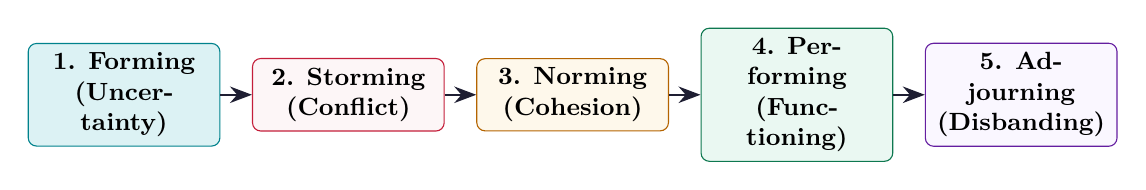
\begin{tikzpicture}[node distance=0.5cm, auto]
  \node [block] (f) {1. Forming\\(Uncertainty)};
  \node [block, right=0.4cm of f, fill=hdrred!40, draw=myred] (s) {2. Storming\\(Conflict)};
  \node [block, right=0.4cm of s, fill=hdramber!50, draw=myamber] (n) {3. Norming\\(Cohesion)};
  \node [block, right=0.4cm of n, fill=hdrgreen!60, draw=mygreen] (p) {4. Performing\\(Functioning)};
  \node [block, right=0.4cm of p, fill=hdrpurple!30, draw=mypurple] (a) {5. Adjourning\\(Disbanding)};

  \draw [arrow] (f) -- (s);
  \draw [arrow] (s) -- (n);
  \draw [arrow] (n) -- (p);
  \draw [arrow] (p) -- (a);
\end{tikzpicture}
\end{tcolorbox}

\begin{enumerate}[leftmargin=*, itemsep=3pt]
  \item \textbf{Forming:} Initial orientation, high uncertainty, testing boundaries and group purpose.
  \item \textbf{Storming:} Intra-group conflict, power struggles, resistance to group constraints.
  \item \textbf{Norming:} Close relationships develop, strong group identity, consensus on norms.
  \item \textbf{Performing:} Group structure becomes fully functional and accepted; focus shifts to task execution.
  \item \textbf{Adjourning:} Disbanding after goal completion (for temporary task groups).
\end{enumerate}

\subsection{Group Behavior: Norms, Cohesiveness, and Roles}
Understanding group behavior requires analyzing three fundamental properties:
\begin{enumerate}[leftmargin=*, itemsep=4pt]
  \item \textbf{Group Norms:} Acceptable standards of behavior shared by group members (performance norms, appearance norms, social arrangement norms).
  \item \textbf{Group Cohesiveness:} The degree to which group members are attracted to each other and motivated to stay in the group.
    \begin{itemize}[leftmargin=*, noitemsep]
      \item \textit{High Cohesiveness + High Performance Norms:} Results in \textbf{highest productivity}.
      \item \textit{High Cohesiveness + Low Performance Norms:} Results in \textbf{low productivity} (group restricts output).
    \end{itemize}
  \item \textbf{Group Conformity \& Asch Effect:} The tendency for members to align their perceptions, opinions, and behaviors with group norms due to social pressure.
\end{enumerate}

% ===============================================================================
% 4. GROUP DECISION MAKING TECHNIQUES AND MERITS/DEMERITS
% ===============================================================================
\section{Group Decision Making: Techniques, Merits, and Demerits}

\subsection{Techniques to Improve Group Decision Making}
\begin{enumerate}[leftmargin=*, itemsep=4pt]
  \item \textbf{Brainstorming:} Idea-generation process encouraging free thinking without criticism.
  \item \textbf{Nominal Group Technique (NGT):} Structured meeting where members write ideas independently before silent voting to prioritize solutions.
  \item \textbf{Delphi Technique:} Systematic decision process collecting anonymous expert opinions via sequential questionnaires without physical meeting.
  \item \textbf{Electronic Meetings:} Combining NGT with computer networking for anonymous real-time voting.
\end{enumerate}

\subsection{Merits and Demerits of Group Decision Making}

\par\vspace{6pt}\noindent
\begingroup
\setlength{\tabcolsep}{5pt}%
\setlength{\extrarowheight}{3pt}%
\renewcommand{\arraystretch}{1.35}%
\begin{tabularx}{\linewidth}{|Y|Y|}
\hline
\multicolumn{1}{|c|}{\textbf{Merits / Advantages}} & \multicolumn{1}{c|}{\textbf{Demerits / Disadvantages}} \\
\hline
\textbf{Complete Information \& Knowledge:} Aggregates diverse expertise, skills, and perspectives. & \textbf{Time-Consuming:} Takes longer to schedule, discuss, and reach consensus compared to individual decisions. \\
\hline
\textbf{Increased Acceptance:} Participants feel ownership, leading to smoother implementation. & \textbf{Groupthink:} Conformity pressure suppresses critical, divergent thinking. \\
\hline
\textbf{Diversity of Views:} Generates more alternatives and creative solutions. & \textbf{Domination by Few:} Vocal or influential members can dominate discussions. \\
\hline
\textbf{Legitimacy:} Democratic consensus decisions are perceived as more legitimate. & \textbf{Ambiguous Responsibility:} Shared accountability dilutes individual responsibility. \\
\hline
\end{tabularx}
\endgroup

% ===============================================================================
% QUICK REVISION PAGE
% ===============================================================================
\newpage
\begin{center}
  {\large\bfseries\color{myred} Quick Revision --- Module 3}\\[3pt]
  {\small\color{mydark} Leadership and Group Dynamics $|$ OE-EC804C}
\end{center}
\vspace{-4pt}
\hrule
\vspace{8pt}

\begin{tcolorbox}[formulabox, title={\textbf{Key Concepts and Metrics at a Glance}}]
\renewcommand{\arraystretch}{1.35}
\begin{tabularx}{\linewidth}{>{\raggedright\arraybackslash\bfseries}p{4.5cm} X}
Manager vs Leader & Positional authority/control (Manager) vs. Personal influence/vision (Leader). \\[4pt]
Managerial Grid & Blake-Mouton 9x9 grid (Optimal style: 9,9 Team Management). \\[4pt]
Tuckman's 5 Stages & Forming $\to$ Storming $\to$ Norming $\to$ Performing $\to$ Adjourning. \\[4pt]
Groupthink & Phenomenon where pressure for conformity overrides critical appraisal of alternatives. \\[4pt]
Delphi Technique & Decision-making technique using anonymous expert questionnaires. \\
\end{tabularx}
\end{tcolorbox}

\begin{tcolorbox}[defbox, title={\textbf{One-Line Definitions for Exam Revision}}]
  \begin{itemize}[leftmargin=*, itemsep=2pt]
    \item \textbf{Transformational Leadership:} Style inspiring followers to transcend self-interest for strategic organizational vision.
    \item \textbf{Group Dynamics:} The social interactions and behavioral forces operating within human groups.
    \item \textbf{Nominal Group Technique:} Structured group decision method restricting discussion during initial idea generation.
    \item \textbf{Groupthink:} Deterioration of mental efficiency and moral judgment resulting from in-group pressures.
  \end{itemize}
\end{tcolorbox}

\begin{tcolorbox}[exambox, title={\textbf{Frequently Asked / Viva Questions}}]
\begin{enumerate}[leftmargin=*, itemsep=4pt]
  \Q{Define Leadership. How does a Leader differ from a Manager?}{Leadership is the ability to influence a group toward achieving a vision. Managers rely on formal authority for stability; Leaders rely on personal influence to drive change.}
  
  \Q{Explain Blake-Mouton's Managerial Grid. Which position represents optimal leadership?}{The grid plots Concern for Production vs. Concern for People on a 9x9 scale. Position (9,9) Team Management is the optimal style.}
  
  \Q{Differentiate between Transactional and Transformational Leadership.}{Transactional leadership relies on contingent exchanges and rewards; Transformational leadership inspires followers to innovate and achieve visionary goals.}
  
  \Q{Trace Tuckman's 5 stages of group development.}{Forming (orientation) $\to$ Storming (conflict) $\to$ Norming (cohesion) $\to$ Performing (functioning) $\to$ Adjourning (disbanding).}
  
  \Q{What is Group Dynamics?}{The social forces, interactions, processes, and behavioral patterns operating within and between human groups.}
  
  \Q{What is Groupthink? How can it be prevented?}{Groupthink is the pressure for conformity suppressing critical dissent. It can be prevented by assigning a devil's advocate and encouraging open feedback.}
  
  \Q{Explain the Delphi Technique of decision making.}{A systematic decision method collecting anonymous opinions from distributed experts via sequential questionnaires without physical meetings.}
  
  \Q{What are the major advantages of group decision making over individual decision making?}{Groups provide more complete information, diverse perspectives, creative alternatives, and higher implementation acceptance.}
  
  \Q{What is a Laissez-Faire leadership style? When is it effective?}{A free-rein style granting complete operational freedom to subordinates. Effective only with highly expert, self-motivated professionals.}
  
  \Q{Describe the characteristic style of leadership in Indian corporate organizations.}{Paternalistic leadership, which combines firm administrative authority with family-like personal care and nurturance.}
\end{enumerate}
\end{tcolorbox}

\end{document}
